\chapter{Metodologia}
\label{cap:metodologia}

\section{Reprodutibilidade}

Esta seção detalha os aspectos técnicos necessários para a reprodução dos experimentos realizados neste trabalho. A implementação segue uma formulação baseada em Processo de Decisão de Markov Parcialmente Observável Descentralizado (Dec-POMDP), com detalhamento do ambiente de simulação, configurações, estados, ações, função de recompensa e toda a estrutura de Curriculum Learning implementada.

\subsection{Formulação Dec-POMDP}

O problema de controle multiagente em futebol de robôs é formulado como um Dec-POMDP, representado pela tupla:

$$G = \langle D, A, S, Z, P, R \rangle.$$

Onde:
\begin{itemize}
    \item $D$: Conjunto de agentes robóticos que participam do jogo;
    \item $A$: Espaço de ações disponíveis para cada agente;
    \item $S$: Espaço de estados do ambiente (não completamente observável pelos agentes);
    \item $Z$: Espaço de observações parciais que cada agente recebe;
    \item $P$: Função de transição que determina a dinâmica do ambiente;
    \item $R$: Função de recompensa que guia o aprendizado dos agentes.
\end{itemize}

A formulação Dec-POMDP é particularmente adequada para este domínio, pois os agentes precisam tomar decisões baseadas em observações locais parciais, enquanto colaboram para alcançar objetivos comuns, como marcar gols e evitar que o adversário marque.

\subsection{Conjunto de Agentes $D$}

O conjunto de agentes varia conforme o estágio do curriculum learning e o tipo de experimento. A configuração padrão para o jogo completo é:

$$D_{azul} = \{d_1, d_2, d_3\}$$ para o time azul e $$D_{amarelo} = \{d_4, d_5, d_6\}$$ para o time amarelo.

O número de agentes é dinamicamente ajustado durante as diferentes fases do curriculum learning:

\begin{itemize}
    \item \textbf{Curriculum Task 0 (Fundamentos Básicos)}: $D_{azul} = \{d_1\}$ e $D_{amarelo} = \{\emptyset\}$ (nenhum agente adversário);
    \item \textbf{Curriculum Task 1 (Interação com Oponentes Estáticos)}: $D_{azul} = \{d_1, d_2, d_3\}$ e $D_{amarelo} = \{d_4\}$ (apenas um agente adversário estático);
    \item \textbf{Self-play}: $D_{azul} = \{d_1, d_2, d_3\}$ e $D_{amarelo} = \{d_4, d_5, d_6\}$ (configuração completa).
\end{itemize}

Todos os agentes de um mesmo time compartilham os mesmos parâmetros de política (policy sharing), o que facilita o aprendizado coletivo e reduz a dimensionalidade do problema. Essa abordagem de compartilhamento de política permite que comportamentos emergentes de coordenação surjam naturalmente durante o treinamento.

\subsection{Espaço de Ações $A$}

Cada agente possui um espaço de ação contínuo com 4 dimensões:

$$a_d = (v_x, v_y, \omega_{\theta}, k) \in [-1.0, 1.0]^4.$$

Onde:
\begin{itemize}
    \item $v_x$: Velocidade normalizada no eixo x (movimento lateral);
    \item $v_y$: Velocidade normalizada no eixo y (movimento frontal);
    \item $\omega_{\theta}$: Velocidade angular normalizada (rotação);
    \item $k$: Ação de chute (contínua, onde valores > 0 executam o chute).
\end{itemize}

Estas ações de alto nível são convertidas para comandos de baixo nível das quatro rodas do robô usando a cinemática do robô omnidirecional. A conversão segue o seguinte processo:

\subsubsection{Transformação de coordenadas}

Primeiro, as velocidades no referencial global são transformadas para o referencial local do robô:
$$v_x', v_y' = v_x \cdot \cos(\theta) + v_y \cdot \sin(\theta), -v_x \cdot \sin(\theta) + v_y \cdot \cos(\theta).$$

Onde $\theta$ é a orientação atual do robô.

\subsubsection{Cálculo das velocidades angulares das rodas}

Em seguida, as velocidades locais e a velocidade angular são convertidas para comandos de velocidade das quatro rodas omnidirecionais:
$$\omega_{roda0} = \frac{v_y'}{r} - \frac{L \cdot \omega_{\theta}}{r}.$$
$$\omega_{roda1} = \frac{v_x'}{r} + \frac{L \cdot \omega_{\theta}}{r}.$$
$$\omega_{roda2} = -\frac{v_y'}{r} - \frac{L \cdot \omega_{\theta}}{r}.$$
$$\omega_{roda3} = -\frac{v_x'}{r} + \frac{L \cdot \omega_{\theta}}{r}.$$

Onde $r$ é o raio das rodas e $L$ é a distância do centro do robô até as rodas.

\subsubsection{Desnormalização e limitação}

Os valores normalizados são desnormalizados para as velocidades físicas reais:
\begin{itemize}
    \item Velocidades lineares são multiplicadas por 1.5 m/s
    \item Velocidade angular é multiplicada por 10 rad/s
\end{itemize}

Os valores resultantes são limitados às velocidades máximas permitidas pelos atuadores do robô. Esta abordagem permite que os agentes aprendam comportamentos complexos emergentes, como driblar, passar e defender, a partir deste conjunto de ações de baixo nível.

\subsection{Espaço de Estados $S$}

O estado completo $S$ do ambiente representa todas as informações físicas do sistema simulado, incluindo:

\begin{itemize}
    \item Posição $(x, y)$ e orientação $\theta$ de todos os robôs;
    \item Velocidades lineares $(v_x, v_y)$ e angulares $\omega$ de cada robô;
    \item Posição $(x, y)$ e velocidade $(v_x, v_y)$ da bola;
    \item Estado dos atuadores (velocidades das rodas);
    \item Forças e interações físicas entre todos os objetos do ambiente;
    \item Informações sobre limites do campo, área de gol e outras regiões relevantes.
\end{itemize}

Este estado completo é gerenciado pelo simulador RL-SSL-EL, que implementa a física do ambiente. No entanto, os agentes não têm acesso direto a todas essas informações, apenas a um conjunto de observações parciais derivadas do estado completo, muitas vezes com ruído adicionado para simular imperfeições sensoriais.

A formulação como Dec-POMDP é particularmente adequada neste contexto, pois reconhece que cada agente tem uma visão parcial e potencialmente ruidosa do ambiente, precisando tomar decisões com informação incompleta, semelhante ao problema enfrentado por robôs reais em um jogo físico.

\subsection{Espaço de Observações $Z$}

Cada agente $d$ recebe uma observação parcial $z_d \in Z$ do estado do ambiente. Esta observação é um vetor de 77 valores que inclui informações relevantes para a tomada de decisão do agente. Para capturar aspectos temporais e dinâmicos do jogo, estas observações são empilhadas com as 7 observações anteriores, resultando em um vetor final de entrada com 616 valores (8 × 77).

O vetor de observação é composto pelas seguintes categorias de informação:

\subsubsection{Posições Cartesianas}
\begin{itemize}
    \item Posição $(x, y)$ normalizada do próprio robô relativa ao centro do campo;
    \item Posições $(x, y)$ normalizadas dos companheiros de time relativas ao centro do campo;
    \item Posições $(x, y)$ normalizadas dos adversários relativas ao centro do campo;
    \item Posição $(x, y)$ normalizada da bola relativa ao centro do campo.
\end{itemize}

\subsubsection{Orientações Angulares}
\begin{itemize}
    \item Seno e cosseno da orientação do próprio robô para representação contínua sem descontinuidades;
    \item Arcotangente da orientação do próprio robô como informação complementar;
    \item Seno, cosseno e arcotangente dos ângulos formados entre o robô e seus aliados;
    \item Seno, cosseno e arcotangente dos ângulos formados entre o robô e os adversários;
    \item Seno, cosseno e arcotangente dos ângulos formados entre a bola e o centro de cada gol.
\end{itemize}

\subsubsection{Distâncias Euclidianas}
\begin{itemize}
    \item Entre o robô e cada companheiro de time;
    \item Entre o robô e cada adversário;
    \item Entre o robô e a bola;
    \item Entre a bola e ambos os gols (aliado e adversário).
\end{itemize}

\subsubsection{Informações Temporais e Contextuais}
\begin{itemize}
    \item Ações anteriores de todos os companheiros de time no tempo $t-1$;
    \item Tempo restante no episódio (normalizado para o intervalo $[0,1]$).
\end{itemize}

Todas as observações são normalizadas para o intervalo $[-1.0, 1.0]$ para facilitar o treinamento da rede neural. A normalização é realizada dividindo os valores brutos por constantes específicas para cada tipo de dado:
\begin{itemize}
    \item Posições: divididas pelo tamanho máximo do campo;
    \item Distâncias: divididas pela diagonal do campo;
    \item Velocidades: divididas pelas velocidades máximas permitidas.
\end{itemize}

O empilhamento temporal de 8 frames a 10Hz (correspondendo a 0.8 segundos de jogo) permite que o agente infira informações sobre velocidades e trajetórias, mesmo sem acesso direto a estes dados. Esta representação do estado foi cuidadosamente projetada para fornecer ao agente informações suficientes para tomar decisões tático-estratégicas eficazes.

\subsection{Função de Transição $P$}

A função de transição $P(s' | s, a)$ representa a dinâmica do ambiente, determinando como o estado $s$ evolui para o próximo estado $s'$ após a execução da ação conjunta $a$ por todos os agentes. No contexto deste trabalho, a dinâmica é implementada pelo ambiente de simulação \textit{RL-SSL-EL}, que oferece simulação física do futebol de robôs, incluindo movimentação dos robôs, dinâmica da bola, e interações entre os agentes no campo.

\subsubsection{Dinâmica Física Simulada}

A simulação inclui todos os aspectos físicos relevantes:

\begin{itemize}
    \item \textbf{Robôs}: Modelados como corpos rígidos com quatro rodas independentes, massa e momento de inércia realistas;
    \item \textbf{Bola}: Modelada como uma esfera com propriedades físicas apropriadas para simulação de deslizamento, rolamento e colisões;
    \item \textbf{Colisões}: Detecção de colisões entre robôs, bola e limites do campo;
    \item \textbf{Atrito}: Implementação de atrito entre diferentes superfícies, tanto estático quanto dinâmico;
    \item \textbf{Mecanismo de chute}: Simulação da força aplicada à bola quando a ação de chute é ativada.
\end{itemize}

\subsubsection{Regras do Jogo}

Além da física pura, a função de transição também implementa as regras específicas do jogo de futebol de robôs:

\begin{itemize}
    \item \textbf{Resets após gol}: Quando um gol é marcado, todos os robôs e a bola são reposicionados para as suas posições iniciais;
    \item \textbf{Resets laterais}: Quando a bola sai pelos limites laterais do campo, os robôs e a bola são reposicionados, mas o episódio continua;
    \item \textbf{Resets de linha de fundo}: Quando a bola sai pelos limites de fundo do campo, os robôs e a bola são reposicionados, mas o episódio continua;
    \item \textbf{Faltas}: Implementação de regras básicas para identificação e penalização de faltas.
\end{itemize}

\subsubsection{Detalhes da Implementação}

A simulação opera com os seguintes parâmetros:

\begin{itemize}
    \item \textbf{Frequência de simulação física}: 30 FPS (frames por segundo) para garantir estabilidade e precisão;
    \item \textbf{Frequência de observação e ação}: 10 Hz para os agentes;
    \item \textbf{Duração dos episódios}: 40 segundos de jogo simulado;
    \item \textbf{Limite de passos por episódio}: Variável conforme o estágio do curriculum (300 a 500 passos)
\end{itemize}

Esta função de transição procura equilibrar o realismo físico necessário para simular adequadamente o futebol de robôs com a eficiência computacional exigida para treinamento em aprendizado por reforço, que requer milhões de interações com o ambiente.

\subsection{Função de Recompensa $R$}

A função de recompensa é um componente crítico do sistema de aprendizado por reforço, pois guia o comportamento dos agentes em direção aos objetivos desejados. Em nosso trabalho, projetamos uma estrutura de recompensa adaptativa que evolui conforme os estágios do curriculum learning, permitindo o desenvolvimento progressivo de habilidades.

\subsubsection{Recompensa Padrão (Self-play)}

No estágio final de Self-play, a recompensa combina elementos contínuos e discretos. A componente contínua $r$ é formada pela soma ponderada de quatro termos:

$$r = 0.7 \cdot r_{speed} + 0.1 \cdot r_{dist} + 0.1 \cdot r_{off} + 0.1 \cdot r_{def}.$$

Onde:

\begin{itemize}
    \item $r_{speed} = \text{clip}\left(\frac{\text{dist}(b_{t-1}, G) - \text{dist}(b_t, G) - 0.05}{0.14}, -1.0, 1.0\right).$
    
    Onde $b_t$ é a posição da bola no tempo $t$, $G$ é a posição do gol adversário, e $\text{dist}()$ é a distância euclidiana. Os fatores $0.05$ e $0.14$ são parâmetros de calibração que estabelecem o limiar mínimo de movimento necessário e a escala de normalização, respectivamente.
    
    \item $r_{dist} = 
    \begin{cases}
      -1, & \text{se } \min(P) \geq 1 \\
      -\min(P), & \text{se } \min(P) < 1
    \end{cases}.$
    
    Onde $P$ é o conjunto das distâncias normalizadas entre cada robô do time e a bola. Esta recompensa incentiva que pelo menos um jogador esteja próximo da bola, penalizando situações onde todos os agentes estão distantes da bola.
    
    \item $r_{off} = \frac{\theta_{RBG}}{\pi} - 1.$
    
    Onde $\theta_{RBG}$ é o ângulo formado pelo robô (R), a bola (B) e o gol adversário (G). Este ângulo é normalizado para o intervalo $[-1.0, 0.0]$, onde valores mais próximos de zero representam posições ofensivas mais vantajosas.
    
    \item $r_{def} = \frac{\theta_{GRB}}{\pi} - 1.$
    
    Onde $\theta_{GRB}$ é o ângulo formado pelo gol aliado (G), o robô (R) e a bola (B). Similar ao $r_{off}$, esta recompensa incentiva posições defensivas eficazes para bloquear possíveis ataques adversários.
\end{itemize}

\subsubsection{Recompensas de Eventos}

Além da recompensa contínua, eventos discretos importantes geram recompensas significativas:

\begin{itemize}
    \item \textbf{Gol marcado}: $+10$;
    \item \textbf{Gol sofrido}: $-10$;
    \item \textbf{Bola fora do campo}: $-1$.
\end{itemize}

Estes valores sobrepõem-se à recompensa contínua quando ocorrem, criando sinais fortes para guiar o aprendizado em momentos críticos.

\subsubsection{Recompensas Específicas do Curriculum Learning}

Cada estágio do curriculum possui ajustes específicos na função de recompensa, adaptados aos objetivos pedagógicos de cada fase:

\begin{itemize}
    \item \textbf{Curriculum Task 0 (Fundamentos Básicos):}
    \begin{itemize}
        \item \textbf{Recompensa principal}: $+10.0$ quando o robô toca na bola pela primeira vez;
        \item \textbf{Recompensa de aproximação}: $-dist(robô, bola)$, incentivando a aproximação contínua à bola;
        \item \textbf{Penalidade por tempo}: $-0.01$ por passo, incentivando ações rápidas;
        \item \textbf{Critério de sucesso}: Tocar na bola pelo menos uma vez durante o episódio.
    \end{itemize}
    
    \item \textbf{Curriculum Task 1 (Interação com Oponentes Estáticos):}
    \begin{itemize}
        \item \textbf{Proximidade da bola}: $-0.1 \times dist(robô\_mais\_próximo, bola)$;  
        \item \textbf{Posse de bola}: $+0.05 \times \min(frames\_com\_posse / 30, 1.0)$, recompensando o controle contínuo da bola;
        \item \textbf{Aproximação do gol}: $+0.3 \times (1 - dist\_normalizada(bola, gol\_adversário))$;
        \item \textbf{Gol marcado}: $+10.0$;
        \item \textbf{Gol sofrido}: $-10.0$;
        \item \textbf{Penalidade por sair do campo}: $-1.0$ (robô), $-0.5$ (bola);
        \item \textbf{Critério de sucesso}: Marcar pelo menos um gol durante o episódio.
    \end{itemize}
\end{itemize}

Esta estrutura de recompensa progressiva permite que os agentes desenvolvam habilidades em uma sequência pedagógica eficaz, facilitando o aprendizado de comportamentos complexos a partir de capacidades fundamentais mais simples. A transição suave entre os diferentes regimes de recompensa é essencial para o sucesso da abordagem de curriculum learning implementada.

\subsection{Curriculum Learning}

O Curriculum Learning implementado neste trabalho consiste em uma abordagem estruturada e progressiva para o aprendizado de habilidades complexas em futebol de robôs. Diferentemente da abordagem tradicional de Self-play, onde os agentes enfrentam diretamente o ambiente completo, o curriculum divide o aprendizado em estágios sequenciais de complexidade crescente, facilitando o desenvolvimento gradual de competências.

\subsubsection{Estrutura do Curriculum}

Nosso curriculum foi cuidadosamente projetado com dois estágios principais, cada um focado em um conjunto específico de habilidades fundamentais:

\begin{enumerate}
    \item \textbf{Curriculum Task 0 (Fundamentos Básicos)}: 
    \begin{itemize}
        \item \textbf{Objetivo}: Desenvolver habilidades básicas de navegação e interação com a bola;
        \item \textbf{Configuração}: 1 agente azul sem oponentes em campo;
        \item \textbf{Ambiente}: Campo simplificado com a bola posicionada no centro;
        \item \textbf{Posições iniciais}: Fixas com pequenas variações aleatórias (±0.3 metros);
        \item \textbf{Critério de promoção}: 80\% de sucesso (tocar na bola) em 100 episódios consecutivos;
        \item \textbf{Duração típica}: 55 iterações de treinamento (aproximadamente 20 minutos).
    \end{itemize}
    
    \item \textbf{Curriculum Task 1 (Interação com Oponentes Estáticos)}:
    \begin{itemize}
        \item \textbf{Objetivo}: Desenvolver habilidades de coordenação entre agentes e estratégias ofensivas;
        \item \textbf{Configuração}: 3 agentes azuis contra 1 oponente amarelo estático;
        \item \textbf{Ambiente}: Campo completo com posicionamento tático dos agentes;
        \item \textbf{Posições iniciais}: Semi-aleatórias em configurações taticamente relevantes;
        \item \textbf{Critério de promoção}: 80\% de sucesso (marcar gol) em 100 episódios consecutivos;
        \item \textbf{Duração típica}: 60 iterações de treinamento (aproximadamente 22 minutos).
    \end{itemize}
\end{enumerate}

\subsubsection{Mecanismo de Promoção Adaptativa}

A transição entre os estágios do curriculum é controlada por um sistema de promoção adaptativa implementado na classe \texttt{CurriculumCallback}. Este mecanismo opera da seguinte forma:

\begin{itemize}
    \item Mantém uma janela deslizante dos últimos 100 episódios;
    \item Calcula continuamente a taxa de sucesso com base nos critérios específicos de cada estágio;
    \item Monitora o desempenho dos agentes em todos os ambientes paralelos;
    \item Promove automaticamente para o próximo estágio quando a taxa de sucesso atinge 80%;
    \item Preserva os pesos da política durante a transição, permitindo transferência de conhecimento.
\end{itemize}

\subsubsection{Integração com Self-play}

Após a conclusão do último estágio do curriculum, o sistema transita automaticamente para o treinamento com Self-play, onde os agentes continuam seu desenvolvimento enfrentando versões cada vez mais competentes de si mesmos. Esta integração segue o seguinte processo:

\begin{enumerate}
    \item Os pesos da política treinada com curriculum são utilizados para inicializar tanto a política dos agentes azuis quanto dos agentes amarelos;
    \item O sistema de Self-play é ativado, com atualizações periódicas da política dos agentes amarelos quando os agentes azuis atingem um desempenho superior (diferença de gols ≥ 0.6);
    \item O treinamento continua por 785 iterações adicionais (aproximadamente 7 horas);
    \item As métricas de desempenho são continuamente monitoradas para avaliar a eficácia da abordagem.
\end{enumerate}

\subsection{Implementação do Algoritmo}

Para o treinamento dos agentes, utilizamos o algoritmo Proximal Policy Optimization (PPO), uma abordagem moderna de policy gradient que oferece estabilidade, eficiência e desempenho consistente. A implementação foi realizada utilizando o framework RLlib da biblioteca Ray, que proporciona escalabilidade e distribuição eficiente do processo de treinamento.

\subsubsection{Estrutura da Rede Neural}

A arquitetura neural utilizada consiste em:

\begin{itemize}
    \item \textbf{Rede de política (actor)}: Rede MLP (Multi-Layer Perceptron) com camadas ocultas [300, 200, 100];
    \item \textbf{Função de ativação}: ReLU (Rectified Linear Unit) para todas as camadas ocultas;
    \item \textbf{Rede de valor (critic)}: Rede MLP com mesma estrutura, mas parâmetros independentes;
    \item \textbf{Camada de saída da política}: Parâmetros de distribuição Beta para cada componente da ação, proporcionando ações contínuas limitadas;
    \item \textbf{Camada de saída do valor}: Valor escalar representando a estimativa de retorno.
\end{itemize}

A distribuição Beta foi escolhida para modelar as ações contínuas porque naturalmente limita os valores ao intervalo [0, 1], que são posteriormente remapeados para [-1, 1] para controle dos robôs. Isso proporciona maior estabilidade durante o treinamento, comparado a outras distribuições como a Gaussiana.

\subsubsection{Compartilhamento de Política}

Uma característica importante da implementação é o compartilhamento de parâmetros entre todos os agentes do mesmo time (policy sharing). Isto significa que:

\begin{itemize}
    \item Todos os robôs do time azul compartilham os mesmos parâmetros de rede neural;
    \item O time amarelo, no estágio de self-play, utiliza uma cópia (potencialmente desatualizada) da política do time azul;
    \item Cada agente recebe observações específicas à sua posição, mas processa-as através da mesma política.
\end{itemize}

Este compartilhamento reduz o número de parâmetros a serem aprendidos, acelera o treinamento e facilita a emergência de comportamentos coordenados.

\subsubsection{Hiperparâmetros e Configurações}

Os principais hiperparâmetros utilizados no treinamento foram:

\begin{itemize}
    \item \textbf{Taxa de aprendizado}: 0.0004;
    \item \textbf{Fator de desconto (gamma)}: 0.99;
    \item \textbf{Parâmetro lambda para GAE (Generalized Advantage Estimation)}: 0.95;
    \item \textbf{Coeficiente de entropia}: 0.01 (incentiva exploração);
    \item \textbf{Parâmetro de clipping}: 0.2 (limita mudanças abruptas na política);
    \item \textbf{Batch size}: 96000 amostras (calculado como workers $\times$ envs $\times$ fragment);
    \item \textbf{Mini-batch size}: 24000 amostras (batch/4);
    \item \textbf{Épocas por atualização}: 5;
    \item \textbf{Workers}: 12 processos paralelos;
    \item \textbf{Ambientes por worker}: 4.
\end{itemize}

\subsubsection{Paralelização e Distribuição}

O treinamento foi distribuído para maximizar a eficiência computacional:

\begin{itemize}
    \item Utilização de 12 trabalhadores paralelos, cada um gerenciando 4 ambientes;
    \item Coleta simultânea de experiências em 48 ambientes (12 $\times$ 4);
    \item Processamento em lote de experiências para atualização da política;
    \item Implementação de buffers de experiência para reduzir a correlação entre amostras.
\end{itemize}

\subsubsection{Avaliação Durante Treinamento}

Durante o treinamento, realizamos avaliações periódicas para monitorar o progresso:

\begin{itemize}
    \item A cada 10 iterações, executamos 50 episódios de avaliação;
    \item Durante a avaliação, desativamos a exploração para medir o desempenho da política aprendida;
    \item Registramos métricas como taxa de vitória, número de gols e duração dos episódios;
    \item Estas métricas são visualizadas em tempo real via TensorBoard.
\end{itemize}

A implementação do algoritmo foi cuidadosamente otimizada para garantir eficiência computacional sem sacrificar a qualidade do aprendizado, permitindo treinamento efetivo mesmo com os recursos computacionais disponíveis (CPU AMD Ryzen 7 7700x com 16 núcleos virtuais, 32GB RAM, e GPU NVIDIA GeForce RTX 3090).

\subsection{Self-Play}

O treinamento por Self-play é uma técnica fundamental para desenvolver agentes competitivos em ambientes multiagente, onde a qualidade dos oponentes evolui à medida que o próprio agente melhora. Em nosso trabalho, implementamos um mecanismo de Self-play estruturado para refinar as habilidades dos agentes após a fase de Curriculum Learning.

\subsubsection{Mecanismo de Self-play Implementado}

Nossa implementação do Self-play segue os seguintes princípios:

\begin{itemize}
    \item O time azul (agentes em treinamento ativo) enfrenta o time amarelo (oponentes);
    \item Os oponentes utilizam uma cópia congelada da política do time azul de uma versão anterior;
    \item A política do time azul é atualizada continuamente através do algoritmo PPO;
    \item A política do time amarelo é atualizada discretamente, apenas quando determinados critérios são atingidos.
\end{itemize}

Esta configuração cria um equilíbrio entre estabilidade e desafio: os oponentes são suficientemente estáveis para permitir aprendizado consistente, mas periodicamente atualizados para apresentar novos desafios.

\subsubsection{Critérios de Atualização dos Oponentes}

A decisão sobre quando atualizar a política dos oponentes é crucial para o sucesso do Self-play. Utilizamos um mecanismo baseado em desempenho:

\begin{itemize}
    \item Mantemos um contador de pontuação (ScoreCounter) que monitora os resultados das últimas 100 partidas;
    \item Calculamos o escore médio como $(gols\_marcados - gols\_sofridos) / número\_de\_jogos;
    \item Quando o escore médio atinge ou ultrapassa 0.6, consideramos que a política atual é suficientemente superior;
    \item Neste momento, copiamos os pesos da política do time azul para o time amarelo;
    \item Após a atualização, resetamos o contador para reiniciar a avaliação.
\end{itemize}

O limiar de 0.6 foi cuidadosamente escolhido para garantir melhorias significativas antes da atualização, evitando oscilações prematuras que poderiam desestabilizar o treinamento.

\subsubsection{Implementação Técnica}

A lógica de Self-play foi implementada na classe \texttt{SelfPlayUpdateCallback}, que herda de \texttt{DefaultCallbacks} do RLlib. Esta classe realiza as seguintes funções:

\begin{itemize}
    \item Rastreia o desempenho do time azul contra o time amarelo;
    \item Gerencia o contador de pontuação e calcula métricas relevantes;
    \item Executa a transferência de pesos quando os critérios são atendidos;
    \item Registra estatísticas para análise posterior.
\end{itemize}

A cada episódio, a callback atualiza suas estatísticas internas e verifica se os critérios de atualização foram atingidos. Todo este processo é automatizado e ocorre durante o treinamento, sem necessidade de intervenção manual.

\subsubsection{Integração com Curriculum Learning}

Na abordagem combinada proposta neste trabalho, a fase de Self-play inicia após a conclusão do curriculum. Esta integração apresenta características específicas:

\begin{itemize}
    \item A política inicial para ambos os times (azul e amarelo) é derivada do modelo treinado no curriculum;
    \item O contador de pontuação é inicializado do zero no início da fase de Self-play;
    \item As primeiras atualizações tendem a ocorrer rapidamente, uma vez que o time azul continua melhorando sobre a base estabelecida pelo curriculum;
    \item À medida que o treinamento avança, as atualizações tornam-se menos frequentes, indicando convergência gradual.
\end{itemize}

\subsubsection{Vantagens Observadas}

Os experimentos demonstraram diversas vantagens do Self-play como mecanismo de refinamento após o Curriculum Learning:

\begin{itemize}
    \item \textbf{Currículo automático}: Cria naturalmente uma progressão de desafios adaptados ao nível do agente;
    \item \textbf{Exploração eficiente}: Incentiva a descoberta de estratégias inovadoras para superar oponentes cada vez mais sofisticados;
    \item \textbf{Robustez aumentada}: Desenvolve políticas que funcionam contra diversas estratégias adversárias;
    \item \textbf{Emergência de comportamentos avançados}: Táticas complexas como passes, posicionamento defensivo e coordenação emergem naturalmente
\end{itemize}

As métricas coletadas durante os experimentos comprovam a eficácia desta abordagem, com o Self-play após Curriculum Learning superando significativamente o Self-play puro em todas as métricas relevantes.

\subsection{Condições de Finalização do Episódio}

A definição de quando um episódio termina é crucial para o aprendizado eficiente, pois determina o horizonte temporal com que os agentes lidam. Em nosso trabalho, um episódio é encerrado quando uma das seguintes condições é satisfeita:

\begin{itemize}
    \item \textbf{Gol marcado}: Um gol é marcado por qualquer uma das equipes;
    \item \textbf{Tempo máximo}: O limite de 40 segundos (1200 passos de simulação a 30 fps) é atingido.
\end{itemize}

É importante distinguir entre a finalização de um episódio e os "resets" durante o episódio. Quando a bola sai do campo (pelas laterais ou linhas de fundo), ocorre um reset das posições dos jogadores e da bola para configurações pré-definidas, mas o episódio continua em andamento, mantendo-se o placar e o tempo decorrido. O sistema registra estas ocorrências como "resets laterais" ou "resets de linha de fundo".

\subsection{Ambiente de Simulação}

O ambiente de simulação utilizado neste trabalho é o \textit{RL-SSL-EL}\footnote{\url{https://github.com/Werikcyano/RL-SSL-EL}} na versão de implementação da equipe de robótica Pequi Mecânico, conforme ilustrado na Figura \ref{fig:campo_simulacao}. Esta plataforma foi projetada especificamente para o futebol de robôs na categoria \textit{Small Size League - Entry League (SSL-EL)}, simplificando o processo de aprendizado por reforço aplicado ao futebol de robôs.

\subsubsection{Características Técnicas}

\begin{itemize}
    \item \textbf{Integração com RLlib}: Compatibilidade total com o \textit{framework RLlib} para treinamento distribuído;
    \item \textbf{Frequência de simulação}: 30 FPS (frames por segundo);
    \item \textbf{Frequência de observação/ação}: 10 Hz para os agentes, representando o ciclo de percepção-ação;
    \item \textbf{Duração máxima do episódio}: 40 segundos (1200 passos de simulação);
    \item \textbf{Dimensões do campo}: Conforme especificações oficiais da categoria SSL-EL;
    \item \textbf{Modelagem dos robôs}: Baseada nas especificações físicas do Pequi Mecânico (massa, dimensões, limites de velocidade).
\end{itemize}

\subsubsection{Modificações para Curriculum Learning}

O ambiente base foi estendido para suportar os diferentes estágios do curriculum learning, com implementações específicas:

\begin{itemize}
    \item \textbf{Classe SSLCurriculumEnv}: Estende o ambiente base com funcionalidades necessárias para o curriculum;
    \item \textbf{Configuração dinâmica}: Permite alteração do número de agentes, posicionamento e regras durante o treinamento;
    \item \textbf{Funções de recompensa adaptativas}: Diferentes sinais de recompensa para cada estágio do curriculum;
    \item \textbf{Sistema de monitoramento}: Métricas específicas para avaliar o progresso em cada estágio.
\end{itemize}

\subsubsection{Visualização}

O ambiente inclui um módulo de visualização baseado em OpenGL que permite a renderização do campo, robôs e bola para inspeção visual durante o treinamento e avaliação. Esta visualização pode ser ativada através da flag \texttt{--evaluation} durante o treinamento.

\subsection{Configuração Computacional}

Os experimentos foram realizados em uma máquina com a seguinte configuração:

\begin{itemize}
    \item \textbf{CPU}: AMD Ryzen 7 7700x com 16 núcleos virtuais;
    \item \textbf{RAM}: 32GB DDR5;
    \item \textbf{GPU}: NVIDIA GeForce RTX 3090 com 24GB de VRAM;
    \item \textbf{Armazenamento}: SSD NVMe de 2TB;
    \item \textbf{Sistema Operacional}: Ubuntu 22.04 LTS.
\end{itemize}

Para reprodução dos experimentos, recomenda-se uma configuração mínima de:

\begin{itemize}
    \item CPU com pelo menos 8 núcleos lógicos;
    \item 16GB de RAM;
    \item GPU com suporte a CUDA e pelo menos 8GB de VRAM;
    \item 100GB de espaço em disco para armazenar checkpoints e logs.
\end{itemize}

\subsubsection{Paralelização e Tempo de Treinamento}

O treinamento distribuído foi configurado com:

\begin{itemize}
    \item 12 workers em paralelo;
    \item 4 ambientes por worker;
    \item Total de 48 ambientes simultâneos.
\end{itemize}

Com esta configuração, o tempo total de treinamento foi aproximadamente:

\begin{itemize}
    \item \textbf{Curriculum + Self-play (abordagem proposta)}: total de 900 iterações
    \begin{itemize}
        \item \textbf{Curriculum Task 0}: 20 minutos (55 iterações);
        \item \textbf{Curriculum Task 1}: 22 minutos (60 iterações);
        \item \textbf{Self-play após Curriculum}: 7 horas (785 iterações);
        \item \textbf{Tempo total}: 7.7 horas (900 iterações).
    \end{itemize}
    \item \textbf{Full Self-play (baseline)}: 8.7 horas (900 iterações)
\end{itemize}

É importante ressaltar que ambas as abordagens utilizaram o mesmo critério de parada: 900 iterações totais de treinamento. Esta equivalência garante uma comparação justa entre os métodos, evidenciando que a abordagem de Curriculum + Self-play fez em menos tempo (7.7 horas versus 8.7 horas).

Todas as configurações específicas, scripts auxiliares e documentação detalhada estão disponíveis no repositório do projeto. Para facilitar a reprodução, fornecemos também um container Docker com todas as dependências pré-configuradas.


\subsection{Visão Geral da Arquitetura do \textit{Curriculum}}

A arquitetura do \textit{curriculum learning} implementada neste trabalho segue uma estrutura de estágios progressivos, onde cada estágio representa um nível de complexidade específico no aprendizado do futebol de robôs. A progressão entre estes estágios é controlada por critérios de desempenho predefinidos, garantindo que os agentes desenvolvam as habilidades necessárias antes de avançar para desafios mais complexos.

A transição do cenário curricular é projetada para preservar a continuidade do aprendizado, evitando mudanças abruptas que poderiam prejudicar o desenvolvimento dos agentes. Esta arquitetura foi inspirada em sistemas de treinamento progressivo observados em jogos eletrônicos populares, como FIFA e \textit{Rocket League}, onde os jogadores são introduzidos gradualmente a conceitos mais complexos. A Figura \ref{fig:diagrama_curriculum} ilustra o fluxo completo do processo de treinamento com \textit{curriculum learning}, destacando as etapas e transições entre os diferentes estágios do aprendizado.

\begin{figure}[H]
    \centering
    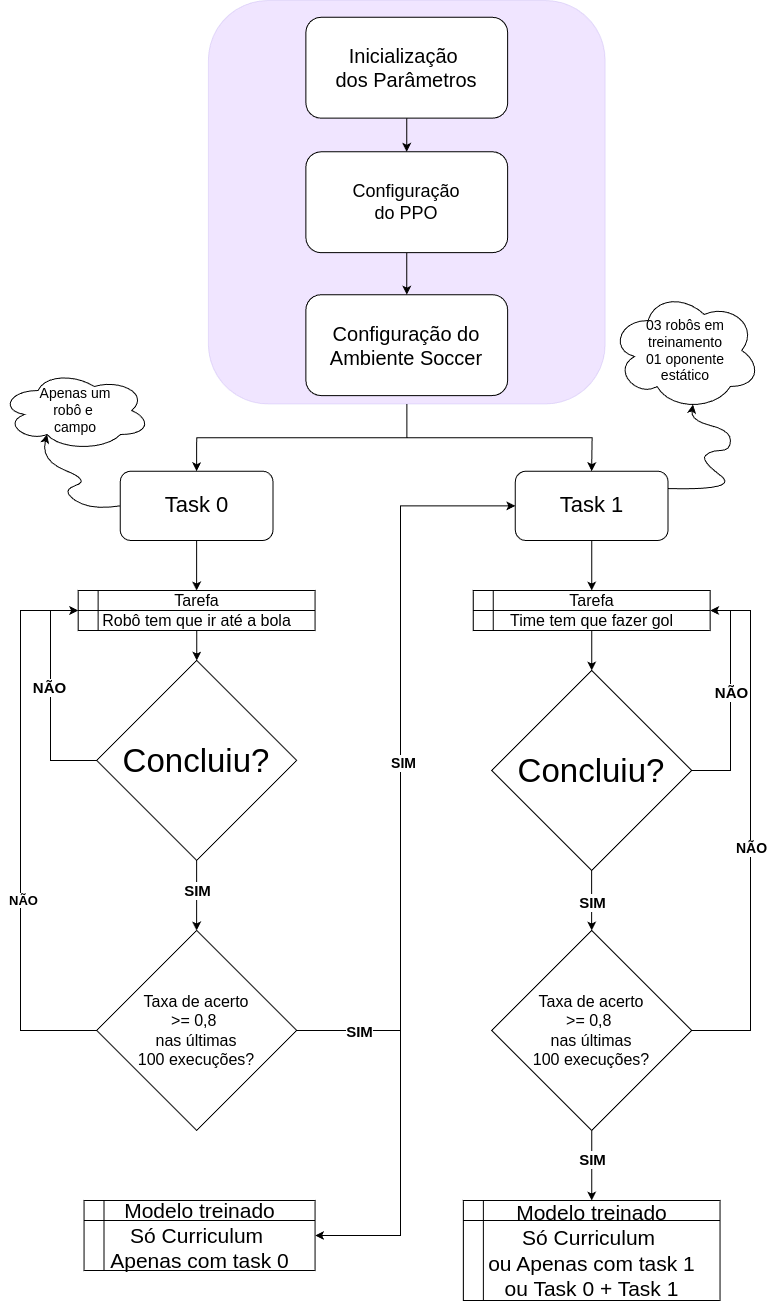
\includegraphics[width=0.85\textwidth]{fig/fluxograma_treino_curriculum.png}
    \caption{Diagrama de fluxo do processo de treinamento com \textit{curriculum learning}. Fonte: Elaborado pelo autor.}
    \label{fig:diagrama_curriculum}
\end{figure}

O fluxo do processo inicia com a definição dos estágios e seus respectivos parâmetros no arquivo de configuração \texttt{config.yaml}. Estes parâmetros incluem critérios de sucesso, sistemas de recompensa específicos, e configurações do ambiente para cada estágio. Durante o treinamento, o \texttt{CurriculumCallback} monitora continuamente o desempenho dos agentes, calculando a taxa de sucesso com base em uma janela deslizante de episódios recentes. Quando esta taxa atinge o limiar de promoção predefinido, o sistema avança automaticamente para o próximo estágio do \textit{curriculum}.


%\subsubsection{Estágio 3 (\textit{Task} 2): Jogo Completo com Oponentes Ativos}
%\label{subsubsec:estagio3}

%O Estágio 3 representa o nível mais avançado do \textit{curriculum}, introduzindo múltiplos oponentes ativos e aproximando-se das condições reais de jogo. Neste estágio, os agentes precisam demonstrar capacidades táticas complexas e coordenação de equipe.

%\paragraph{Configuração do Ambiente}

%O ambiente neste estágio apresenta complexidade máxima:
%\begin{itemize}
%    \item Três robôs da equipe azul, com posicionamento tático
%    \item Três robôs oponentes (equipe amarela), distribuídos estrategicamente pelo campo
%    \item Posições iniciais configuradas para simular situações táticas realistas
%    \item Limite de 500 passos por episódio
%\end{itemize}

%\paragraph{Sistema de Recompensas}

%O sistema de recompensas é refinado para valorizar aspectos estratégicos do jogo:
%\begin{itemize}
%    \item Manutenção das recompensas por proximidade à bola e ao gol
%    \item Valorização adicional de comportamentos defensivos quando necessário
%    \item Penalizações por violações das regras (saída da bola, faltas)
%    \item Recompensas por posicionamento tático eficiente
%\end{itemize}




%\subsubsection{Parâmetros de Configuração}

%Os parâmetros de configuração do \textit{curriculum} são definidos no arquivo \texttt{config.yaml}, utilizando uma estrutura hierárquica que permite especificar detalhadamente as características de cada estágio. Os principais parâmetros incluem:

%\begin{itemize}
%    \item \texttt{enabled}: Flag para ativar ou desativar o \textit{curriculum learning}
%    \item \texttt{initial\_task}: Estágio inicial do \textit{curriculum} (0, 1, ou 2)
%    \item \texttt{promotion\_threshold}: Taxa de sucesso necessária para avançar para o próximo estágio (padrão: 0.8)
%    \item \texttt{evaluation\_window}: Número de episódios para avaliar o desempenho (padrão: 100)
%    \item \texttt{tasks}: Dicionário contendo as configurações específicas de cada estágio:
%    \begin{itemize}
%        \item \texttt{max\_steps}: Limite de passos por episódio
%        \item \texttt{num\_agents\_blue} e \texttt{num\_agents\_yellow}: Número de agentes em cada equipe
%        \item \texttt{init\_pos}: Posições iniciais dos robôs e da bola
%        \item \texttt{reward\_weights}: Pesos das diferentes componentes da recompensa
%        \item \texttt{success\_criteria}: Critérios para considerar um episódio bem-sucedido
%    \end{itemize}
%\end{itemize}

%Esta estrutura de configuração oferece grande flexibilidade para ajustar o \textit{curriculum} de acordo com necessidades específicas, permitindo experimentação com diferentes progressões de aprendizado.

\section{Métricas de Avaliação}
\label{sec:metricas_avaliacao}

Para avaliar o desempenho dos agentes e comparar a eficácia das abordagens de treinamento, foi desenvolvido um conjunto abrangente de métricas que captura diferentes aspectos do comportamento dos agentes. Estas métricas são coletadas durante o treinamento e utilizadas para análises comparativas.

%\subsection{Número de Gols}

%O número de gols marcados representa uma das métricas mais diretas de desempenho no futebol de robôs. Esta métrica é registrada tanto por episódio quanto de forma acumulada ao longo do treinamento, permitindo avaliar a evolução da capacidade ofensiva dos agentes. As submétrias relacionadas incluem:

%\begin{itemize}
%    \item Gols marcados por episódio
%    \item Gols sofridos por episódio
%    \item Percentual de episódios com pelo menos um gol
%    \item Diferença líquida de gols
%\end{itemize}

%Estas métricas fornecem insights sobre a eficácia ofensiva e defensiva dos agentes, aspectos fundamentais do desempenho no futebol de robôs.

\subsection{Tempo dos Episódios}

O tempo dos episódios é uma métrica importante para avaliar a eficiência do jogo e a capacidade dos agentes de alcançar seus objetivos rapidamente. Esta métrica é analisada em diferentes dimensões:

\begin{itemize}
    \item Duração média dos episódios (em passos);
    \item Evolução da duração ao longo do treinamento;
    \item Distribuição dos tempos de episódio.
\end{itemize}

Um aspecto particularmente relevante desta métrica é sua relação com a progressão do treinamento. Tipicamente, espera-se que episódios mais curtos indiquem agentes mais eficientes na realização de seus objetivos.

\subsection{Métrica de Continuidade}

As métricas de continuidade foram desenvolvidas especificamente para este trabalho, visando avaliar a fluidez do jogo e a capacidade dos agentes de manter a bola em jogo por períodos prolongados. Estas métricas incluem:

\begin{itemize}
    \item Número total de \textit{resets} durante todo o treinamento;
    \item Média de \textit{resets} por episódio.
\end{itemize}

Estas métricas são particularmente importantes para avaliar a qualidade do jogo produzido pelos agentes, uma vez que um jogo com menos interrupções tende a ser mais dinâmico e interessante.

%\subsection{Posse de Bola}

%A posse de bola é uma métrica táctica importante que reflete a capacidade dos agentes de controlar o jogo. Para esta análise, são considerados os seguintes aspectos:

%\begin{itemize}
%    \item Percentual de posse de bola por equipe
%    \item Duração média das sequências de posse
%    \item Correlação entre posse e resultados (gols)
%    \item Distribuição espacial da posse no campo
%\end{itemize}

%A análise desta métrica permite compreender as estratégias emergentes dos agentes e sua eficácia em diferentes contextos do jogo.

\subsection{Recompensa Acumulada}

A recompensa acumulada representa a métrica fundamental do aprendizado por reforço, refletindo diretamente o objetivo de otimização dos agentes. Esta métrica é analisada em várias dimensões:

\begin{itemize}
    \item Recompensa média por episódio;
    \item Evolução da recompensa ao longo do treinamento.
\end{itemize}

A análise da recompensa acumulada permite avaliar a convergência do treinamento e comparar diretamente diferentes abordagens em termos de sua eficácia em otimizar o comportamento dos agentes.

\subsection{Avaliação em Torneio}

Para uma avaliação mais abrangente e objetiva do desempenho dos modelos, será realizado um torneio competitivo entre o modelo \textit{baseline} (treinado com \textit{self-play} padrão) e o modelo proposto (incorporando \textit{curriculum learning}). Este torneio permitirá:

\begin{itemize}
    \item Comparação direta do desempenho em condições controladas;
    \item Avaliação da robustez das estratégias aprendidas;
    \item Análise da consistência dos resultados em múltiplas partidas;
    \item Identificação de possíveis vantagens táticas específicas.
\end{itemize}

O formato do torneio será estruturado para garantir uma avaliação estatisticamente significativa, com múltiplas partidas entre os modelos. Os resultados deste torneio fornecerão evidências importantes sobre a eficácia prática das modificações propostas no processo de treinamento.


Além das métricas específicas descritas anteriormente, também serão utilizadas algumas métricas padrão do aprendizado por reforço:

\begin{itemize}
    \item \textit{Entropy} - Mede a aleatoriedade das ações selecionadas pela política, indicando o nível de exploração do agente;
    \item \textit{Policy Loss} - Quantifica o erro na política atual em relação à política ótima estimada;
    \item \textit{VF Explained} - Indica quanto da variância nas recompensas é explicada pelo modelo de valor, medindo a qualidade das estimativas do valor.
\end{itemize}


